\documentclass[12pt,letterpaper]{article}
\usepackage[utf8]{inputenc}
\usepackage{tikz}
\usetikzlibrary{trees}
\usepackage[spanish, es-nodecimaldot]{babel}
\usepackage{amsmath}
\usepackage{color}
\usepackage{algorithm}
\usepackage[noend]{algpseudocode}
\renewcommand{\algorithmicrequire}{\textbf{Entrada:}}
\renewcommand{\algorithmicensure}{\textbf{Salida:}}
\usepackage{subcaption}
\usepackage{amsfonts}
\usepackage{hyperref}
 \hypersetup{
     colorlinks=true,
     linkcolor=blue,
     filecolor=blue,
     citecolor = blue,      
     urlcolor=cyan,
     }
\usepackage{amssymb}
\usepackage{listings}
\usepackage{color}

\newcommand\var[1]{\, \mathrm{Var}\left\lbrack #1 \right\rbrack}

\newcommand\cov[1]{\, \mathrm{Cov} \left\lbrack #1 \right\rbrack}
\newcommand\pr[1]{\, P \left( #1 \right)}

\newcommand\esp[1]{\, \mathbb{E} \left\lbrack #1 \right\rbrack}
\newcommand\integral[4]{\ensuremath{\int_{#1}^{#2} #3 \, d#4}}

\definecolor{mygreen}{rgb}{0,0.6,0}
\definecolor{mygray}{rgb}{0.5,0.5,0.5}
\definecolor{mymauve}{rgb}{0.58,0,0.82}

\lstset{ 
  backgroundcolor=\color{white},   % choose the background color; you must add \usepackage{color} or \usepackage{xcolor}; should come as last argument
  basicstyle=\footnotesize,        % the size of the fonts that are used for the code
  breakatwhitespace=false,         % sets if automatic breaks should only happen at whitespace
  breaklines=true,                 % sets automatic line breaking
  captionpos=b,                    % sets the caption-position to bottom
  commentstyle=\color{mygreen},    % comment style
  deletekeywords={...},            % if you want to delete keywords from the given language
  escapeinside={\%*}{*)},          % if you want to add LaTeX within your code
  extendedchars=true,              % lets you use non-ASCII characters; for 8-bits encodings only, does not work with UTF-8
  firstnumber=1,                % start line enumeration with line 1000
  frame=single,	                   % adds a frame around the code
  keepspaces=true,                 % keeps spaces in text, useful for keeping indentation of code (possibly needs columns=flexible)
  keywordstyle=\color{blue},       % keyword style
  language=R,                 % the language of the code
  morekeywords={*,...},            % if you want to add more keywords to the set
  numbers=none,                    % where to put the line-numbers; possible values are (none, left, right)
  numbersep=5pt,                   % how far the line-numbers are from the code
  numberstyle=\tiny\color{mygray}, % the style that is used for the line-numbers
  rulecolor=\color{black},         % if not set, the frame-color may be changed on line-breaks within not-black text (e.g. comments (green here))
  showspaces=false,                % show spaces everywhere adding particular underscores; it overrides 'showstringspaces'
  showstringspaces=false,          % underline spaces within strings only
  showtabs=false,                  % show tabs within strings adding particular underscores
  stepnumber=2,                    % the step between two line-numbers. If it's 1, each line will be numbered
  stringstyle=\color{mymauve},     % string literal style
  tabsize=2,	                   % sets default tabsize to 2 spaces
  title=\lstname                   % show the filename of files included with \lstinputlisting; also try caption instead of title
}

\usepackage{amsthm}
\newtheorem{theorem}{Teorema}

\usepackage{graphicx}
\usepackage[inner=1.5 cm, outer = 1.5 cm, top=1 cm, bottom = 1.5 cm]{geometry}
\setlength{\parskip}{3mm}
\title{\textsc{Teorema del límite central}}
\author{\textsc{Fabiola Vázquez}}

\setlength{\parindent}{0cm}
\renewcommand{\lstlistingname}{Código}
\floatname{algorithm}{Algoritmo}
\newtheorem{ej}{Ejercicio}
\newtheorem{defi}{Definición}
\newtheorem{teo}{Teorema}



\begin{document}
\maketitle
\hrule 

\section{Introducción}
En el presente trabajo se busca mostrar algunas aplicaciones del teorema del límite central. Comenzamos por enunciar el teorema, sin su demostración, como aparece en el trabajo de Tsitsiklis y Bertsekas \cite{Bertsekas_Tsitsiklis_2008}:

\begin{teo}
	Sea $X_1, X_2, \dots$ una sucesión de variables aleatorias independientes e idénticamente distribuidas, con media en común $\mu$ y varianza $\sigma^2$. Defina 
	\begin{equation}
		Z_n = \frac{X_1 + \dots + X_n - n\mu}{\sigma \sqrt{n}}.
	\end{equation}
	Entonces, para todo $z$,
	\begin{equation}
		\lim_{n \rightarrow \infty} \pr{Z_n \leq z} = \Phi (z),
	\end{equation}
	donde
	\begin{equation}
		\Phi(z) = \frac{1}{\sqrt{2\pi} } \int_{-\infty}^{z} e^{\frac{-x^2}{2}} \, dx.
	\end{equation}
\end{teo}

\section{Fórmula de Stirling}
La fórmula de Stirling es una útil manera de aproximar el valor de $n!$, y se puede obtener usando el teorema del límite central, como hace Ross \cite{Ross_2000}. La fórmula y su demostración se muestran a continuación:

\begin{teo}[Fórmula de Stirling]
	$n! \approx n^{n + \frac{1}{2}} e^{-n} \sqrt{2 \pi}$.
\end{teo}
\begin{proof}
	Sea $X_1, X_2, \dots$ una sucesión de variables de Poisson independientes, cada una con media 1. Sea $S_n = \sum_{i = 1}^{n} X_i$, y observe que la media y varianza de $S_n$ son ambas iguales a $n$. Entonces, 
	\begin{align}
	\pr{S_n = n} &= \pr{n-1 < S_n \leq n}\\
	&= \pr{-1/\sqrt{n} < (S_n -n)/\sqrt{n} \leq 0}\\
	&\approx \int_{-1/\sqrt{n}}^{0} (2\pi)^{-1/2} e^{-x^2 / 2} \, dx \quad \text{ (cuando } n \text{ es grande, por el teorema del límite central)} \\
	&\approx (2\pi)^{-1/2} (1/\sqrt{n})\\
	&= (2\pi n)^{-1/2}.
	\end{align}
	Pero dado que $S_n$ es Poisson con media $n$, $\pr{S_n = n} = \frac{e^{-n} n^n}{n!}$, así que para $n$ suficientemente grande se tendrá
	\begin{equation}
		\frac{e^{-n} n^n}{n!} \approx (2\pi n)^{-1/2},
	\end{equation} lo cuál es equivalente a la fórmula de Stirling.
\end{proof}

\section{Caminatas aleatorias}

Una caminata aleatoria es un proceso estocástico que describe el movimiento aleatorio de un objeto o partícula. Considere una caminata aleatoria en los enteros. Esto es, empezando en algún entero (cero, por conveniencia), cambiamos de posición hacia la derecha o izquierda con probabilidades $p$ y $1-p$ respectivamente. Al valor $p$ se le suele llamar probabilidad de transición. Cuando $p = 1/2$, esta caminata se dice simétrica. Usando la fórmula de Stirling, Ross \cite{Ross_2000} demuestra que la caminata aleatoria en los enteros regresará un número infinito de veces a su estado inicial si y solo si es simétrica. Un resultado similar se obtiene para una caminata aleatoria simétrica en dos dimensiones, es decir, en la retícula $\mathbb{Z}^2$ con $p = 1/4$ para cualquier dirección. En la figura \ref{fig:caminatas_aleatorias} se muestra la simulación de algunas caminatas aleatorias en los enteros para distintos valores $p$. El experimento se realizó en el software R \cite{R} en un cuaderno de Jupyter \cite{jupyter}.

\begin{figure}
	\centering
	\begin{subfigure}{0.32\linewidth}
		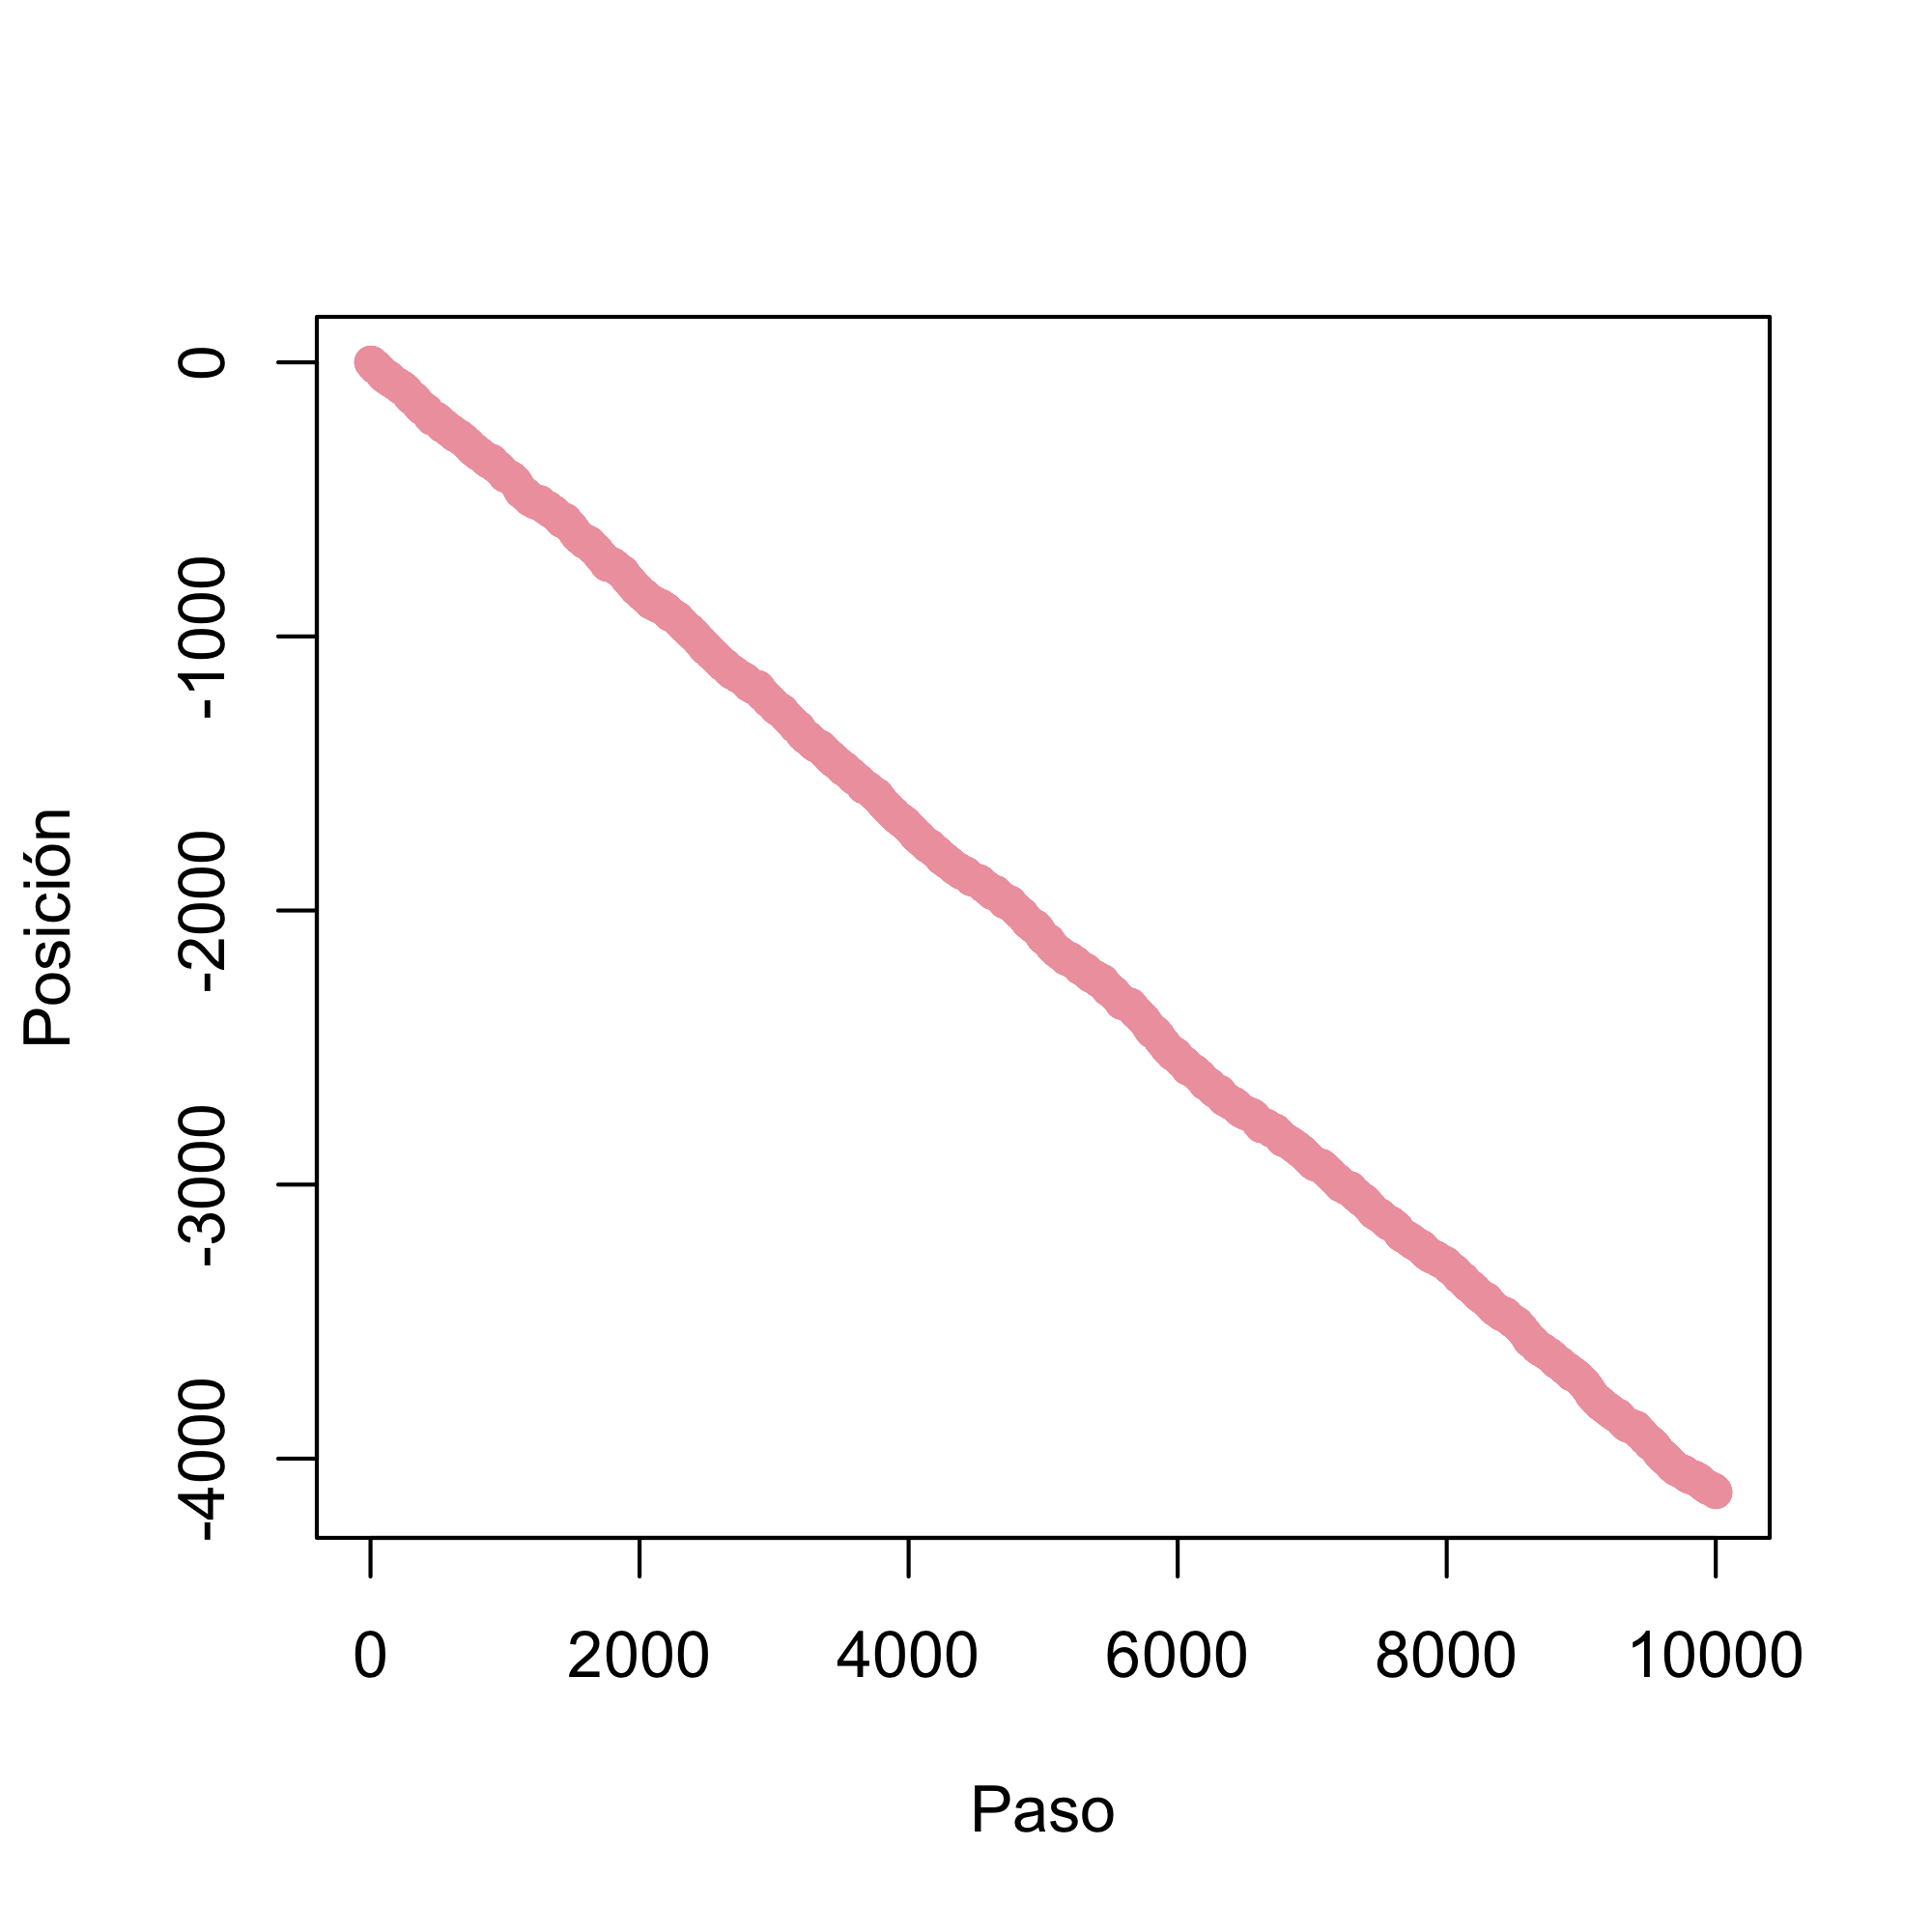
\includegraphics[width=\linewidth]{ca_p3}
		\caption{Caminata aleatoria con $p = 0.3$.}
		\label{fig:ca_p3}
	\end{subfigure}
	\hfill
	\begin{subfigure}{0.32\linewidth}
		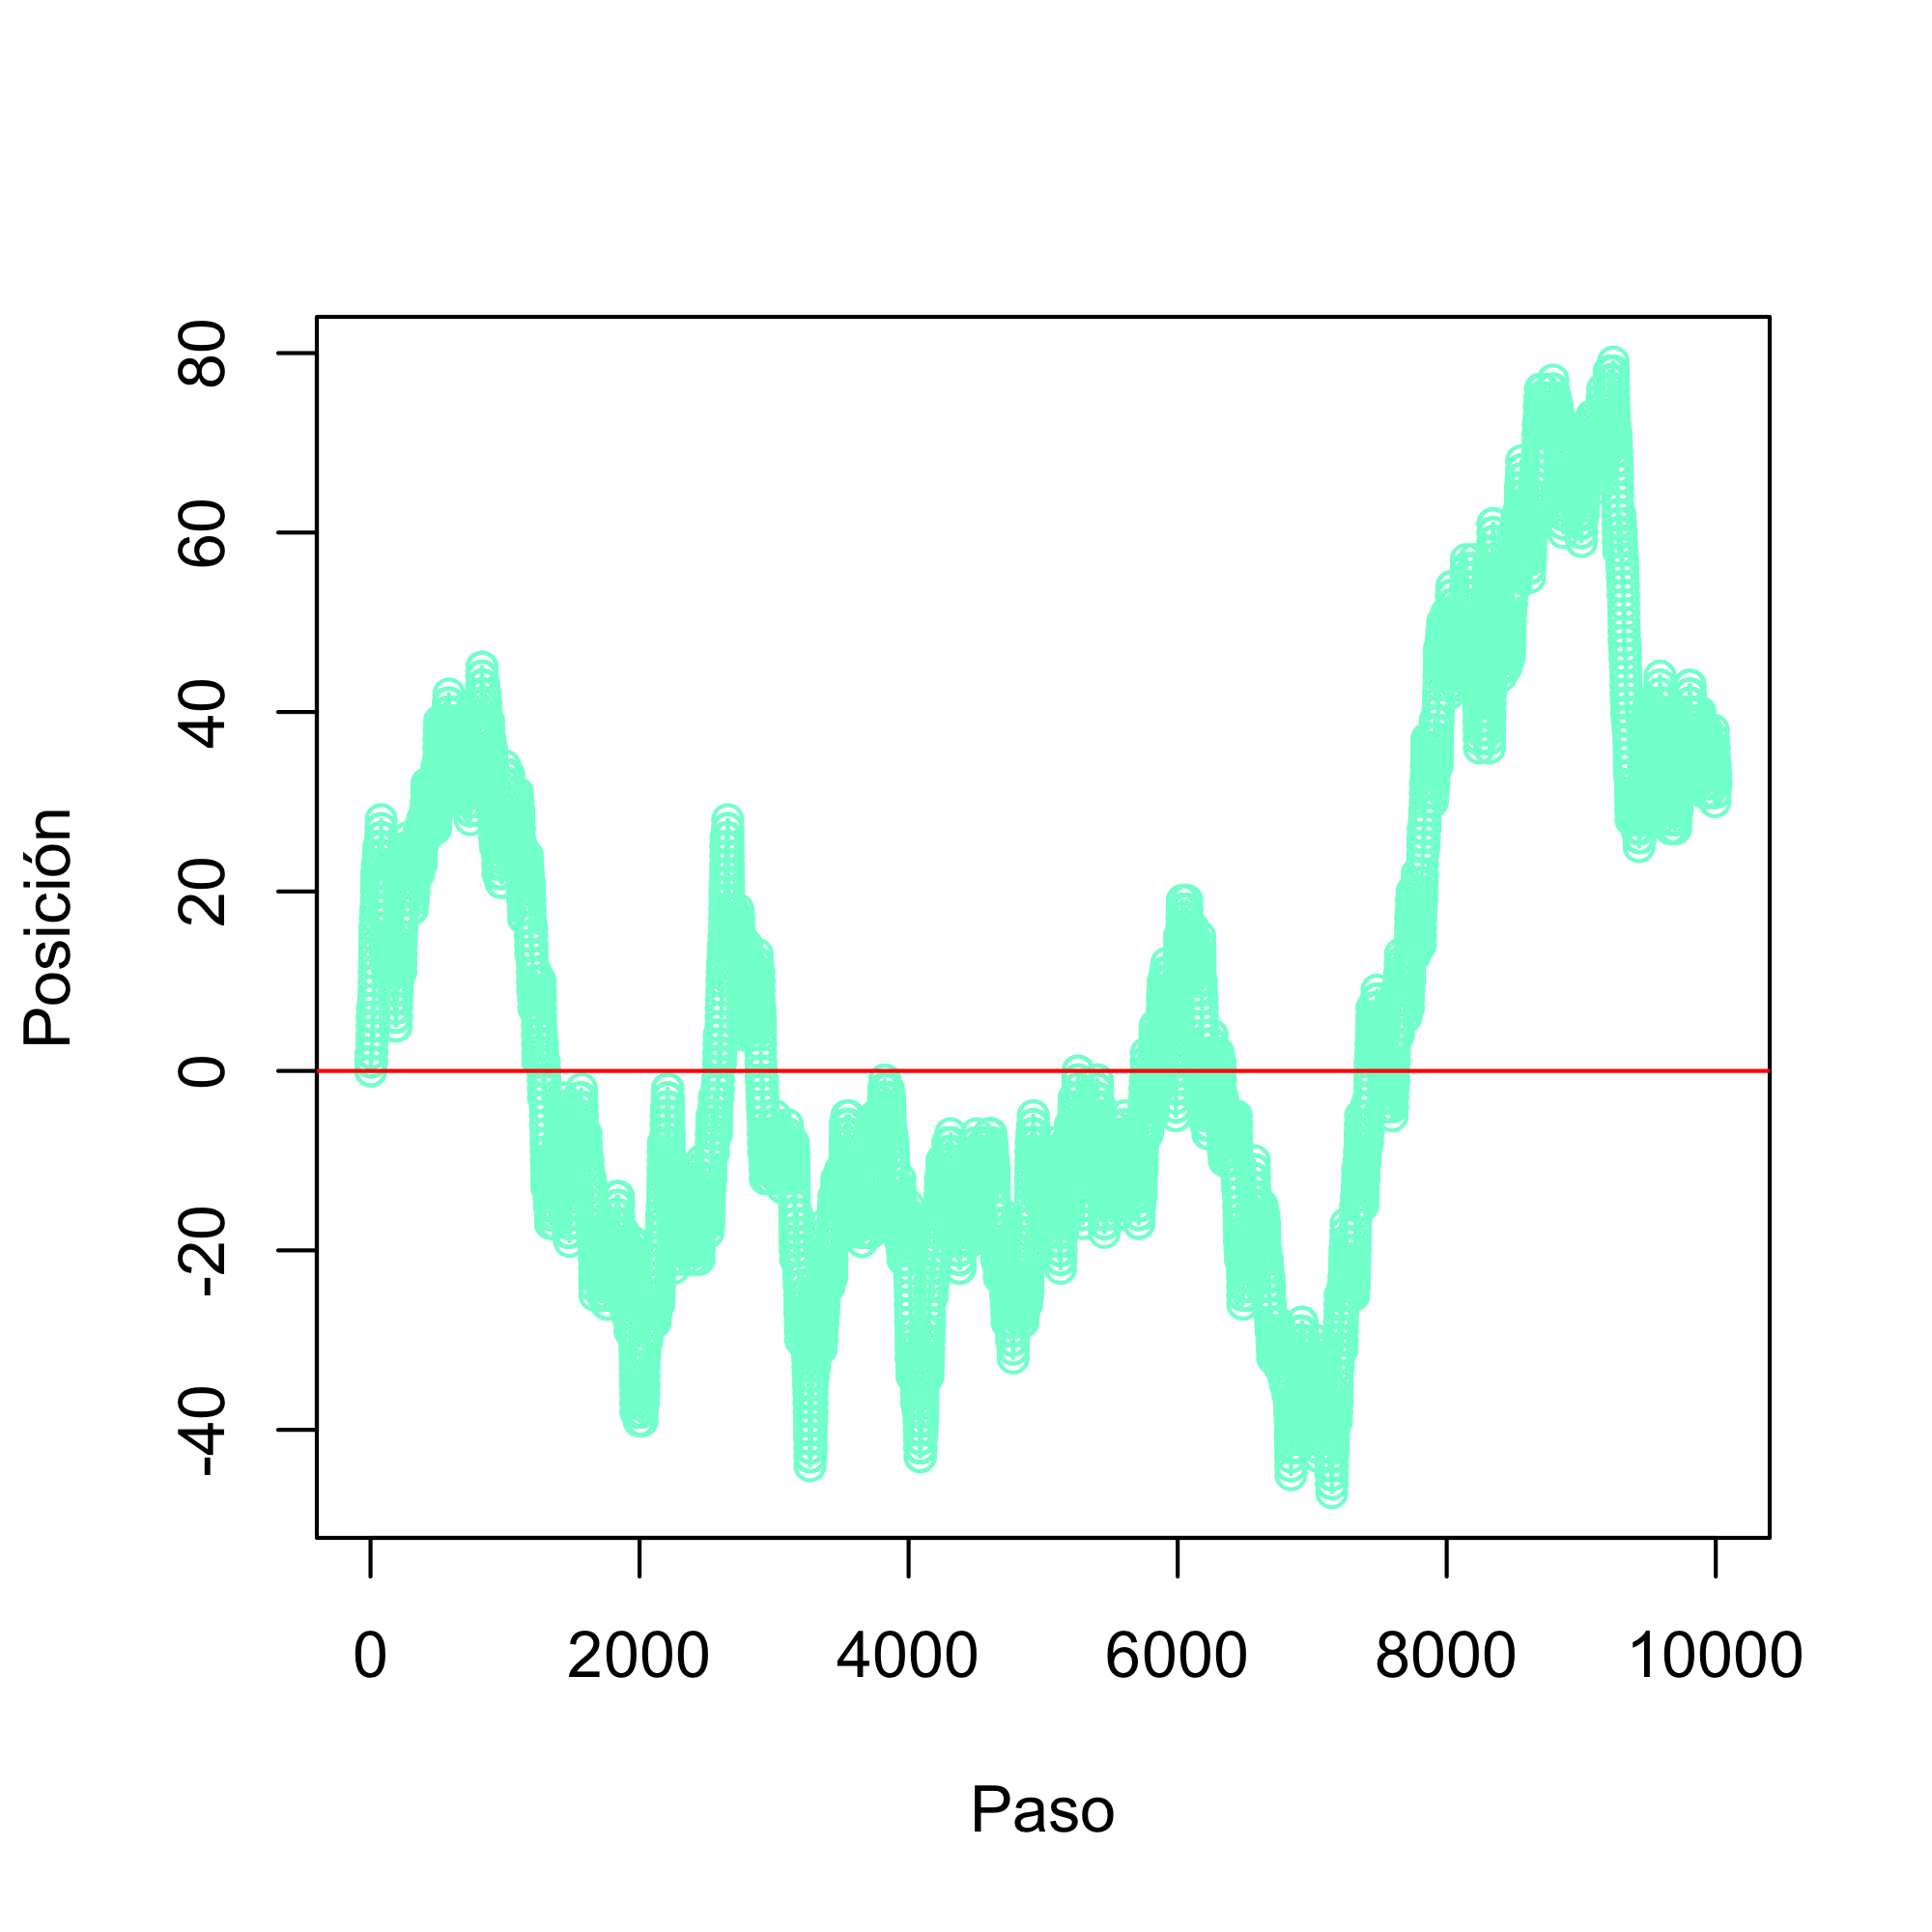
\includegraphics[width=\linewidth]{ca_p5}
		\caption{Caminata aleatoria con $p = 0.5$.}
		\label{fig:ca_p5}
	\end{subfigure}
	\hfill
	\begin{subfigure}{0.32\linewidth}
		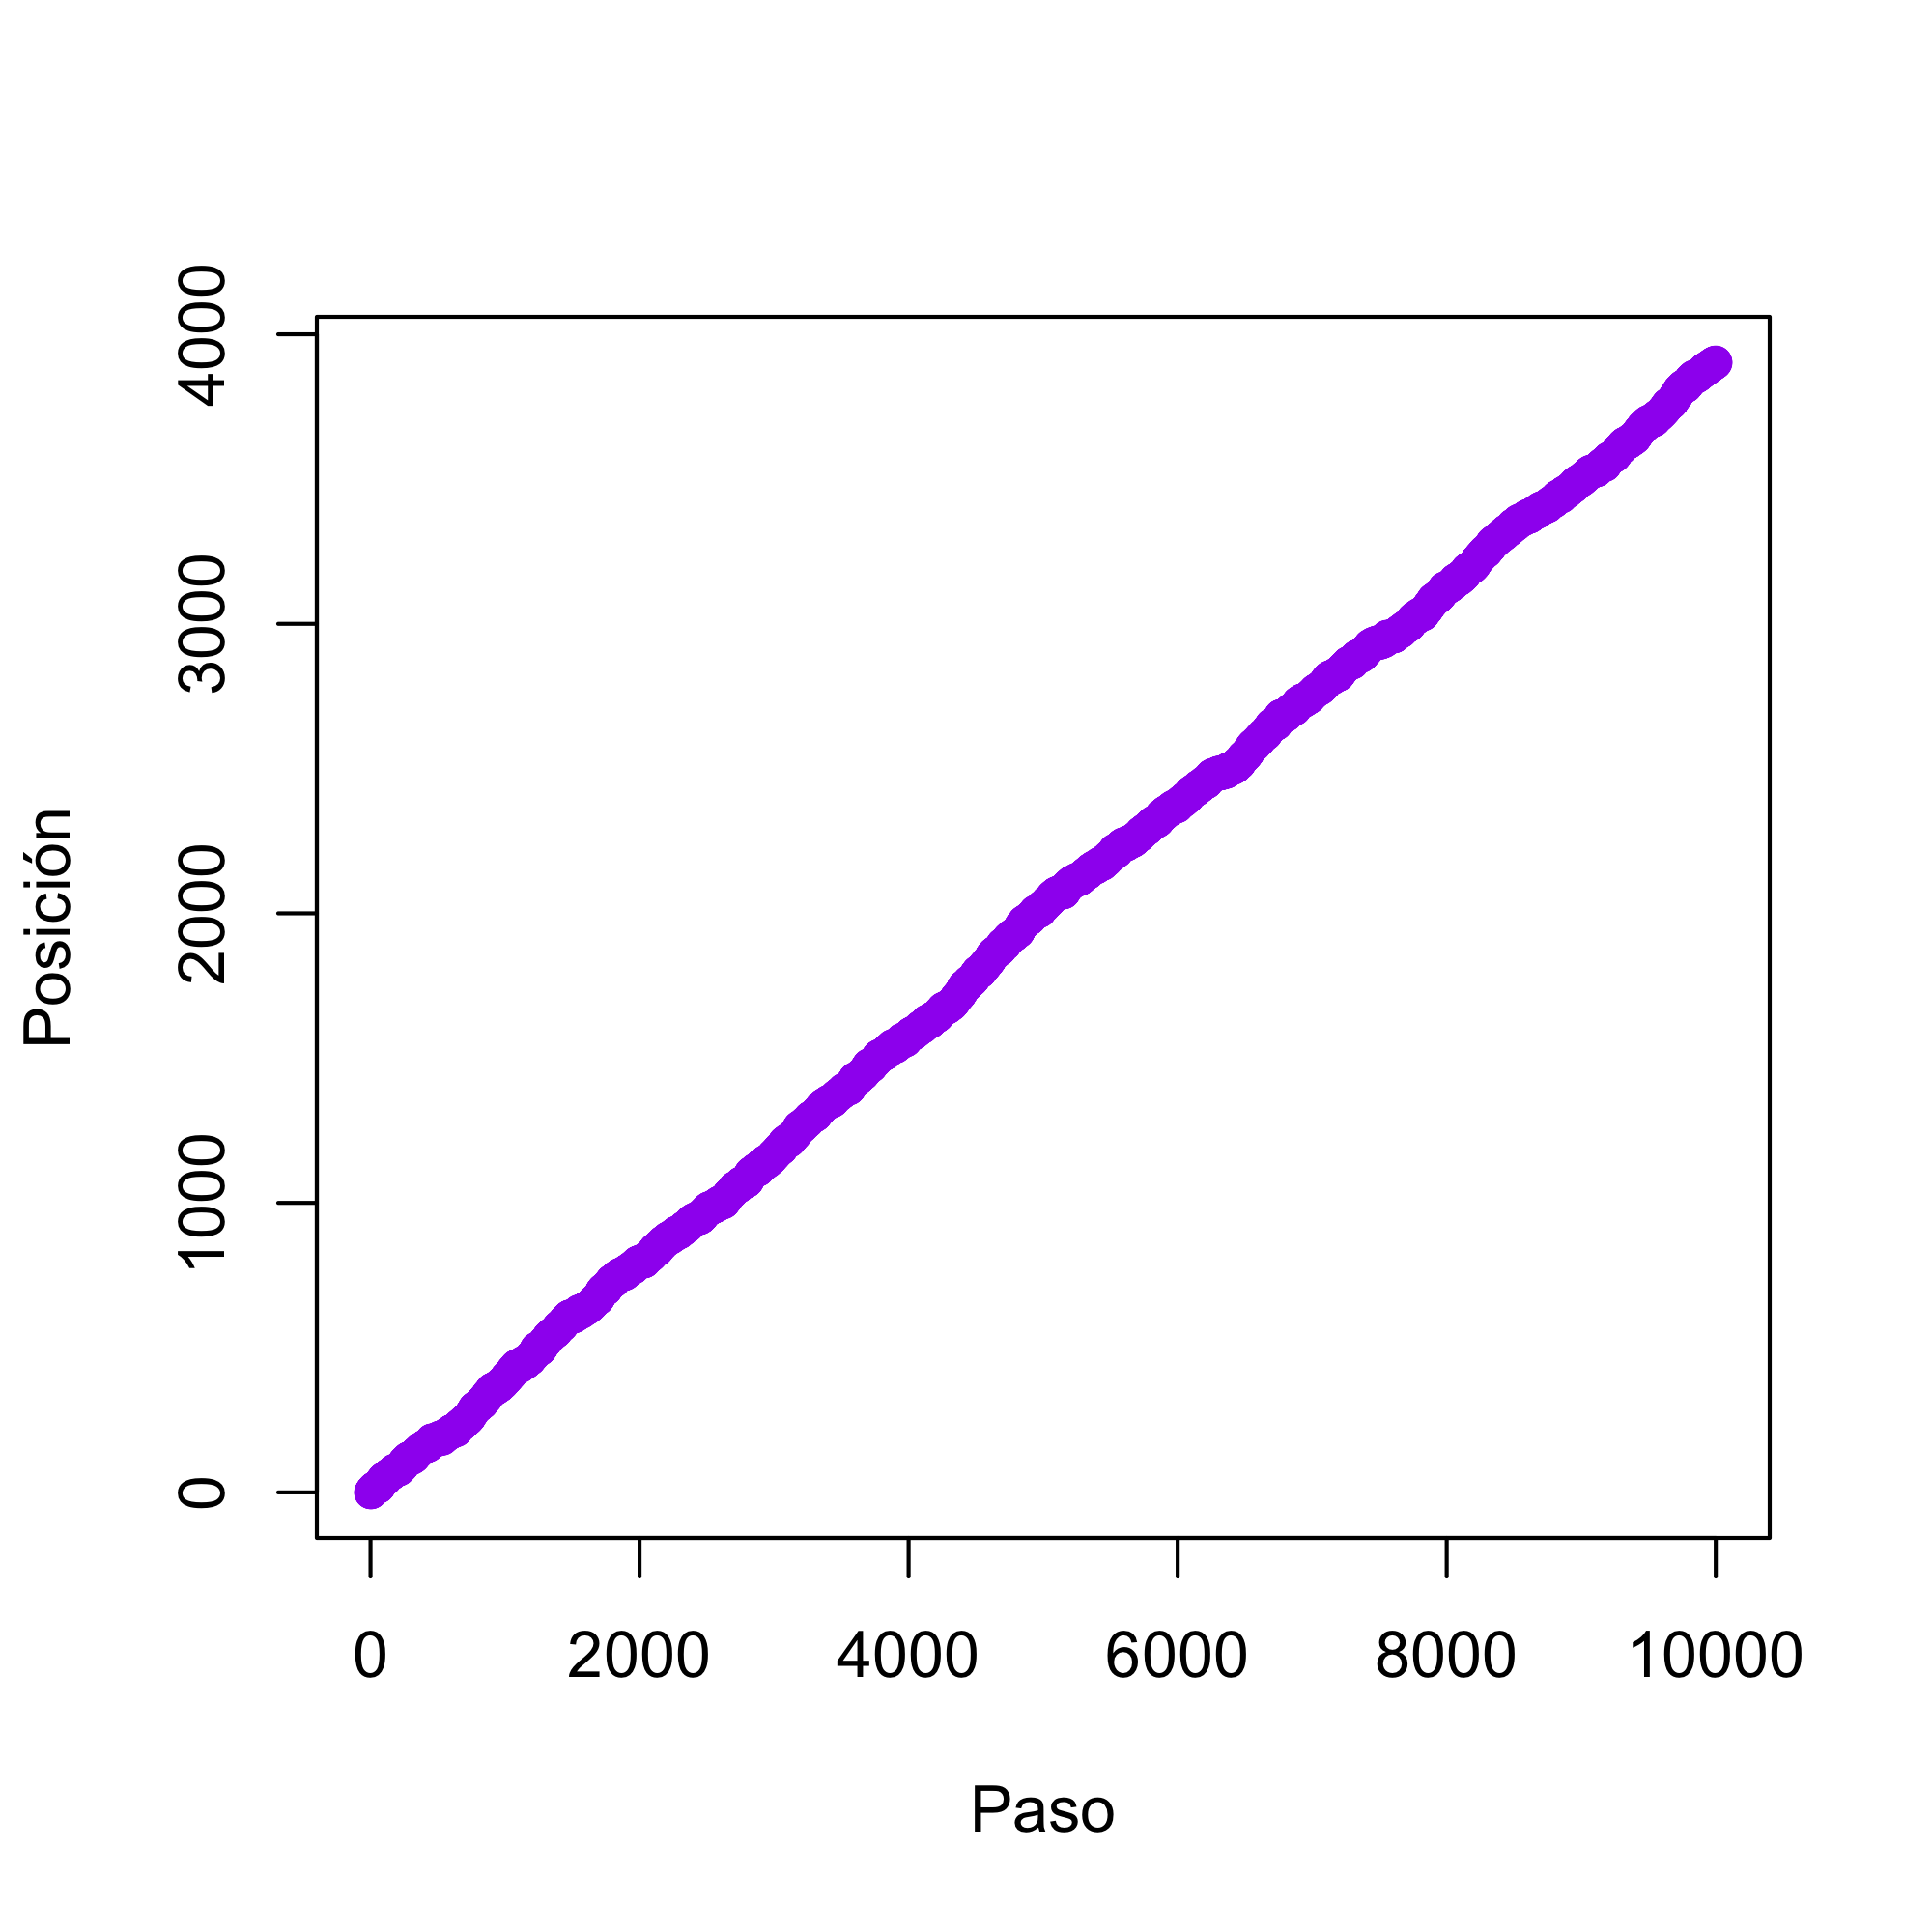
\includegraphics[width=\linewidth]{ca_p7}
		\caption{Caminata aleatoria con $p = 0.7$.}
		\label{fig:ca_p7}
	\end{subfigure}
	\caption{Caminatas aleatorias con distintas probabilidades de transición $p$.} 
	\label{fig:caminatas_aleatorias}
\end{figure}

\subsection{Teorema del límite central para caminatas aleatorias}
Se considera un caso más general, donde el movimiento no está restringido a los enteros, si no a la recta real.  En cada paso $k$, la partícula se desplaza $x_k$ unidades, donde $\lbrace x_k \rbrace$ son variables aleatorias independientes e idénticamente distribuidas. El teorema de límite central para caminatas aleatorias \cite{random_walks_yt} nos dice que, si $\esp{x_k} < \infty$ y $\esp{x_{k}^{2}} < \infty$, la posición $x$ después de $N$ pasos tendrá una distribución normal con media $N \mu$ y varianza $N \sigma^2$, donde cada desplazamiento $x_k$ tiene media $\mu$ y varianza $\sigma^2$. Se realiza una simulación para ejemplificar este teorema. Se simulan mil pasos de una caminata aleatoria cuyos desplazamientos siguen una distribución exponencial con tasa $\lambda=1$, misma que tiene media y varianza 1. Se repite el experimento mil veces, y se analiza la distribución de la última posición en cada caminata, cuyos resultados se muestran en la figura \ref{fig:histogramas}. En la figura \ref{fig:hist_ultima_posicion} se muestra el histograma de la última posición de la caminata, mientras que la figura \ref{fig:hist_normal} se muestra el histograma de números con distribución normal $\mathrm{N}(1000, \sqrt{1000})$. Además de la similitud observada gráficamente, se hizo una prueba de normalidad Shapiro-Wilk, donde los valores de la última posición obtuvieron un valor $p$ de 0.8997. 

\begin{figure}
	\centering
	\begin{subfigure}{0.45\linewidth}
		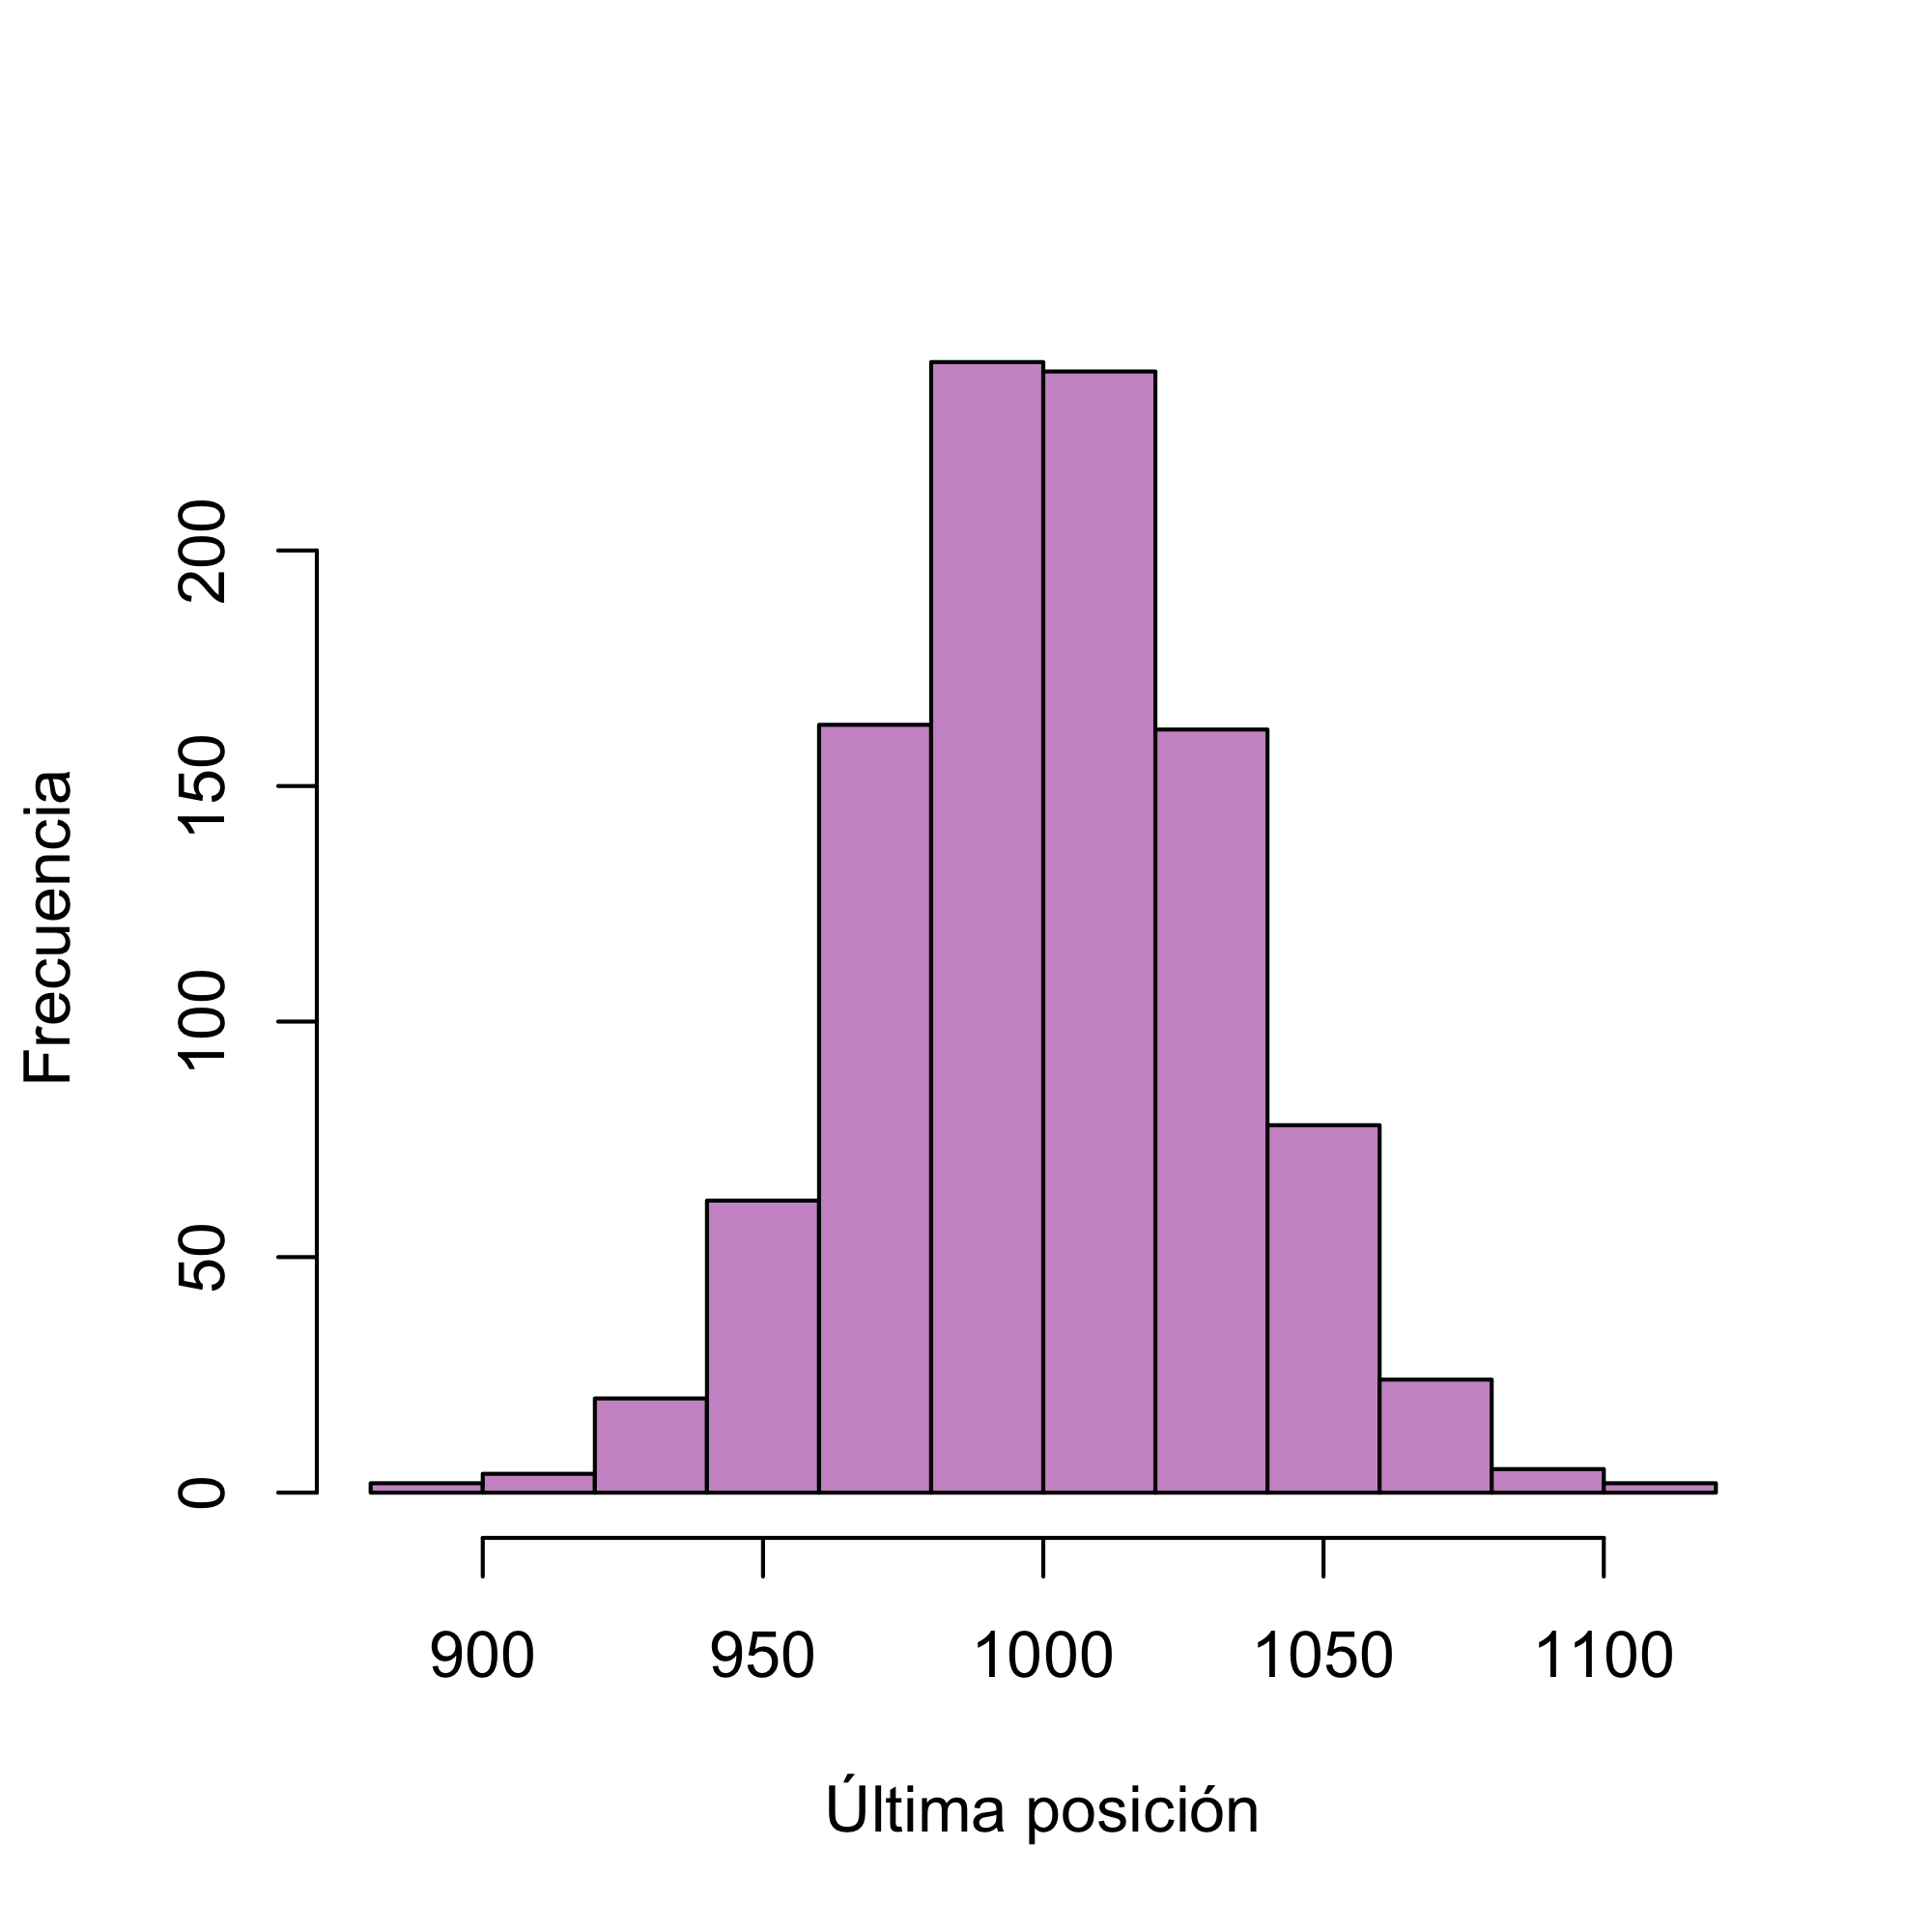
\includegraphics[width=\linewidth]{ultima_posicion}
		\caption{Histograma de la posición de una caminata aleatoria después de mil pasos, con desplazamientos $x \sim \mathrm{Exp}(1)$.}
		\label{fig:hist_ultima_posicion}
	\end{subfigure}
	\hfill
	\begin{subfigure}{0.45\linewidth}
		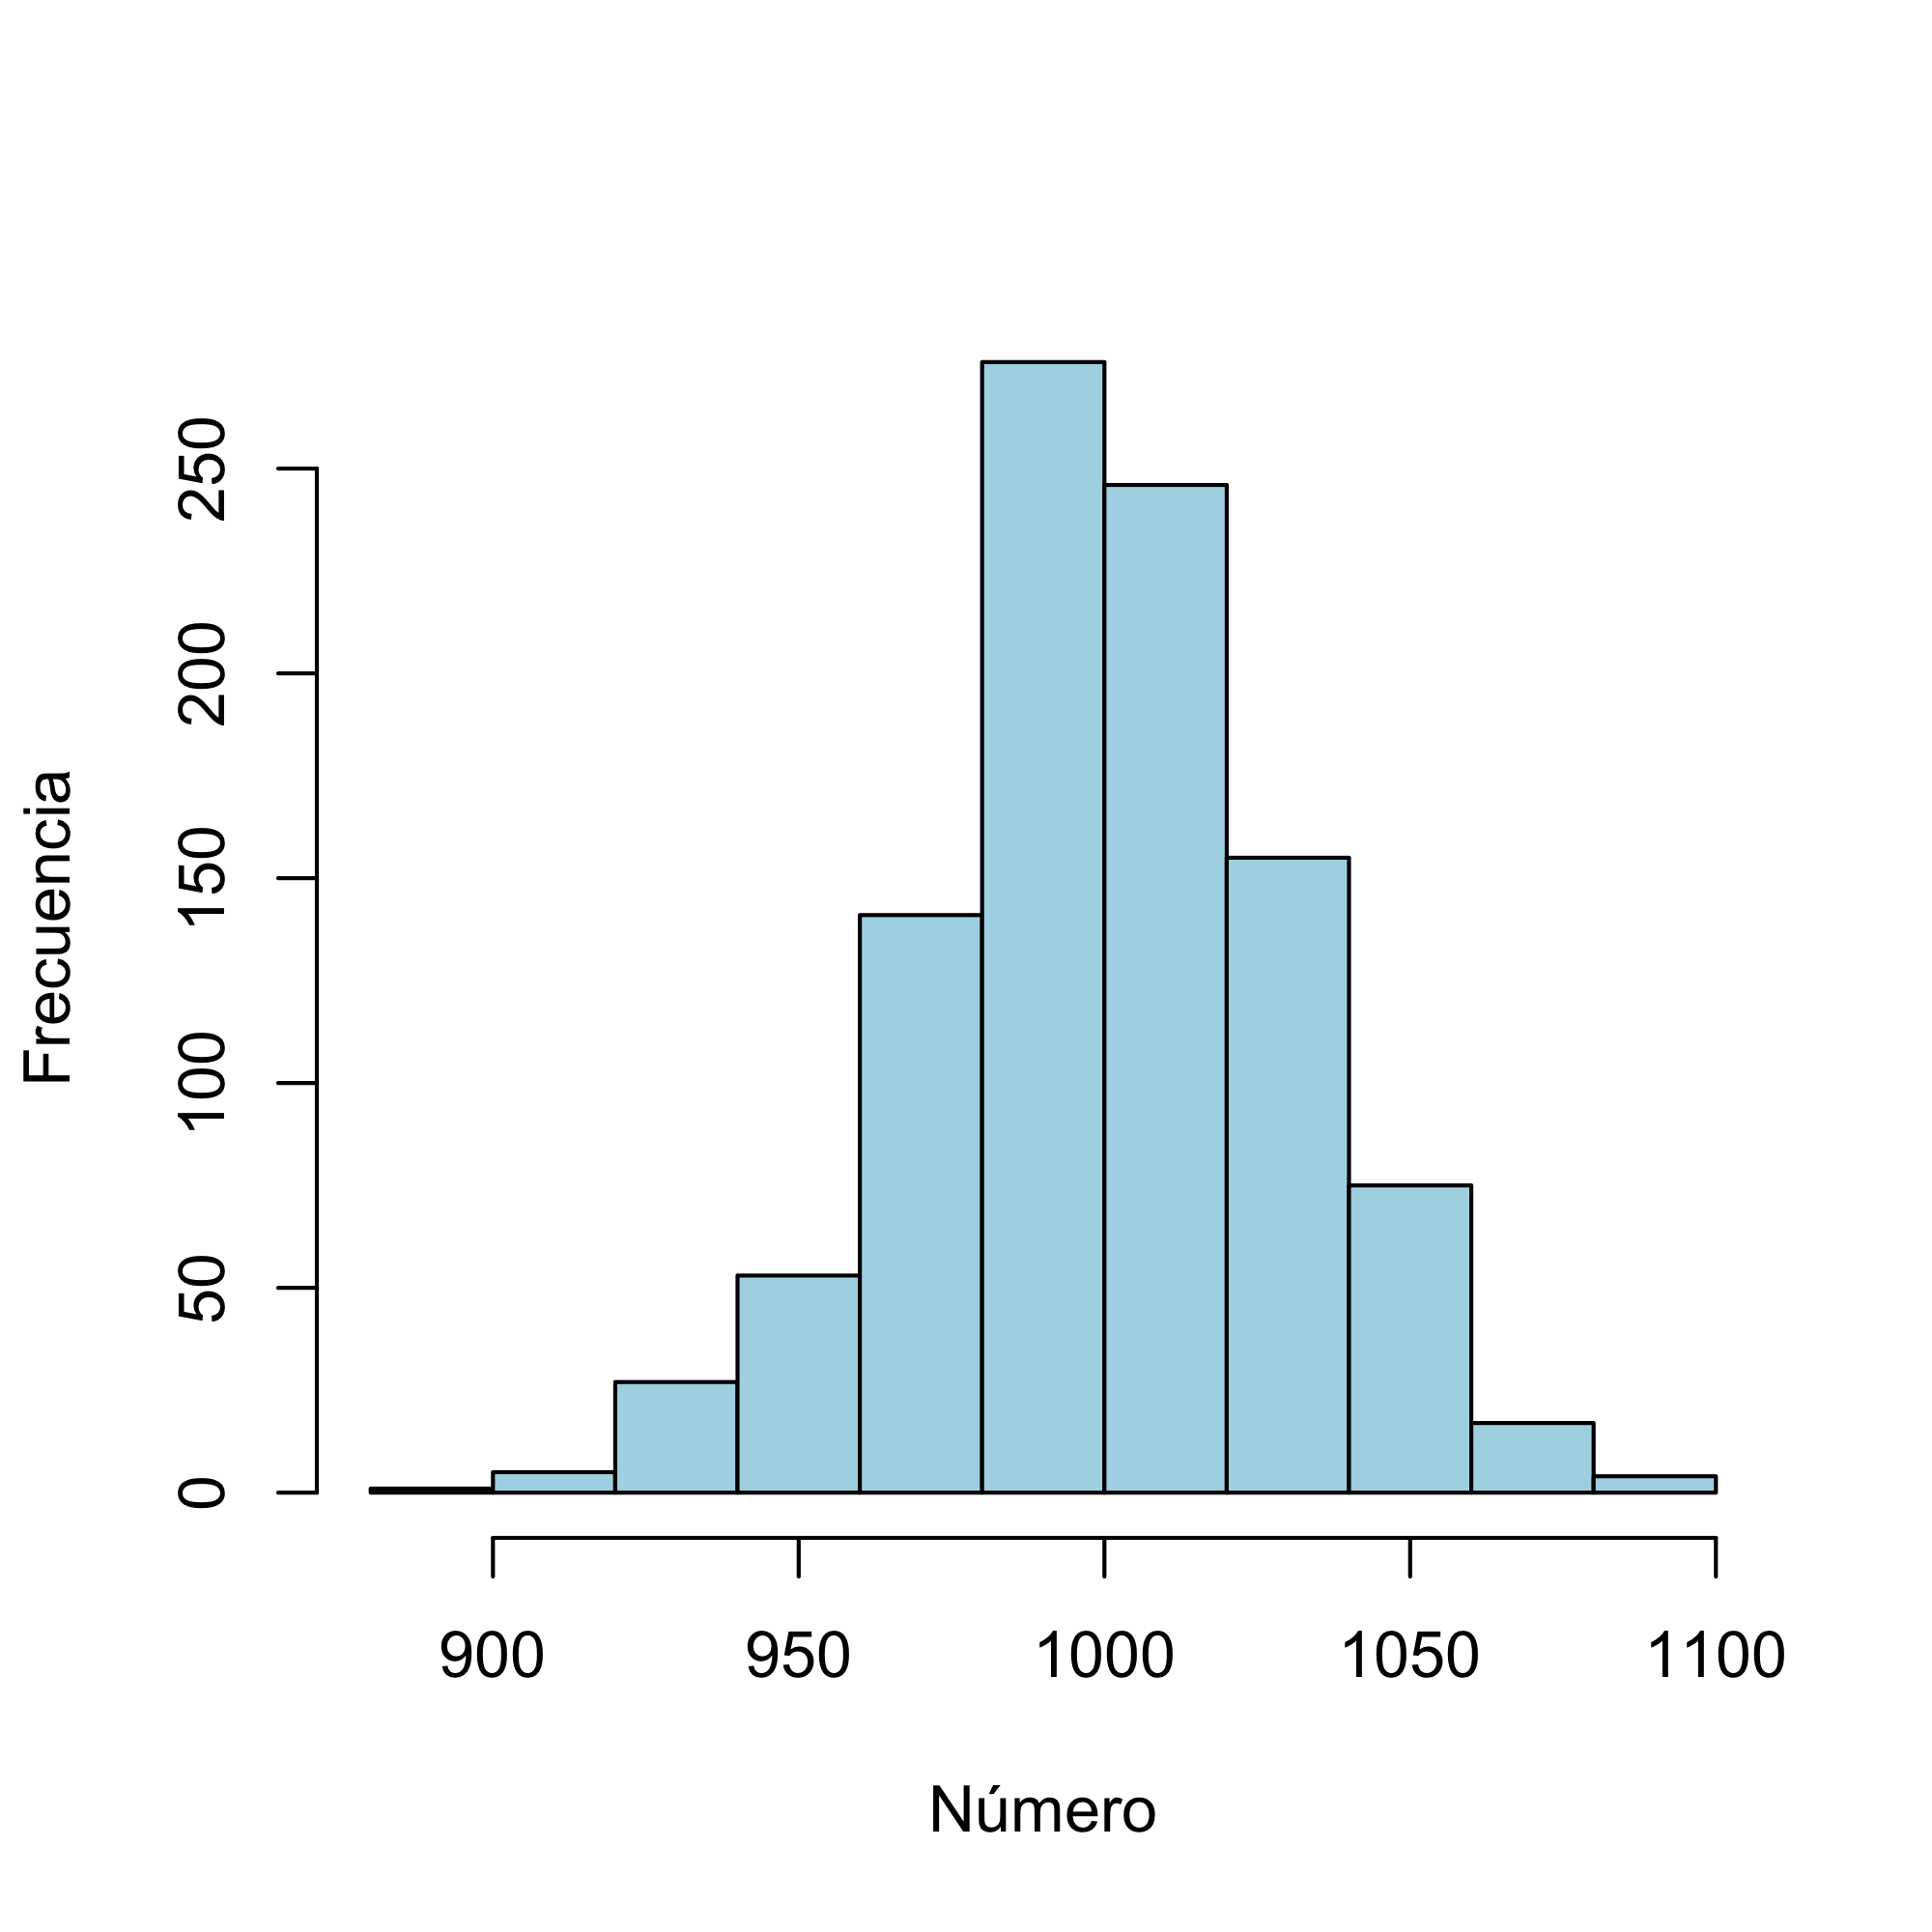
\includegraphics[width=\linewidth]{hist_normal}
		\caption{Histograma de mil números con distribución $\mathrm{N}(1000, \sqrt{1000})$.}
		\label{fig:hist_normal}
	\end{subfigure}
	\caption{Comparación de histogramas de números normales y última posición de una caminata aleatoria.} 
	\label{fig:histogramas}
\end{figure}

\bibliographystyle{plain} 
\bibliography{ref}
\end{document} 